\documentclass[../DS01.tex]{subfiles}%
\graphicspath{{./figures/}}%

% \subimport{/home/nora/Documents/Enseignement/Prepa/bpep/exercices/DS/chimie_du_chrome/}{sujet.tex}%

\begin{document}%
\section[35]"E"{Optique d'un périscope\ifcorrige{~\small\textit{(D'après ENAC 2024)}}}

\enonce{%
	L'entrée d'un périscope est constituée de deux miroirs plans $\Mc_1$ et
	$\Mc_2$, circulaires et de centres respectifs $\mathrm{S_1}$ et $\mathrm{S_2}$
	(Figure~\ref{fig:peri_plain}). Après réflexions réflexions sur $\Mc_1$ et
	$\Mc_2$, la lumière entre dans un système de deux lentilles $\Lc_1$ et
	$\Lc_2$, assimilées à des lentilles minces de centres respectifs
	$\mathrm{O_1}$ et $\mathrm{O_2}$. Les miroirs sont inclinés d'un angle de
	$\ang{45}$ par rapport à l'axe optique du système représenté en pointillés.
	\begin{tcb}[blankest, sidebyside](null){}
		\bigbreak
		L'orientation algébrique de l'axe optique ainsi que celle de l'axe transversal
		sont indiquées sur la figure. Les distances focales images algébriques de
		$\Lc_1$ et $\Lc_2$ sont respectivement $f_1' = \SI{1.0}{m}$ et $f_2' =
			\SI{-0.125}{m}$. Un œil emmétrope (sans défaut) est placé juste derrière
		$\Lc_2$. Le périscope $\Sc_p$ est donc l'ensemble catadioptrique
		$\{\Mc_1,\Mc_2,\Lc_1,\Lc_2\}$. On observe un objet placé dans un plan
		transversal, en avant de $\Sc_p$.
		\bigbreak
		On introduit les distances $a = \mathrm{S_2S_1} > 0$, $b = \mathrm{S_2O_1} >
			0$, $e = \mathrm{O_1O_2} > 0$ et $d = \mathrm{AS_1} > 0$. Dans tout
		l'exercice, on admet que les lentilles fonctionnent dans les conditions de
		\textsc{Gauss}.
		\tcblower
		\begin{center}
			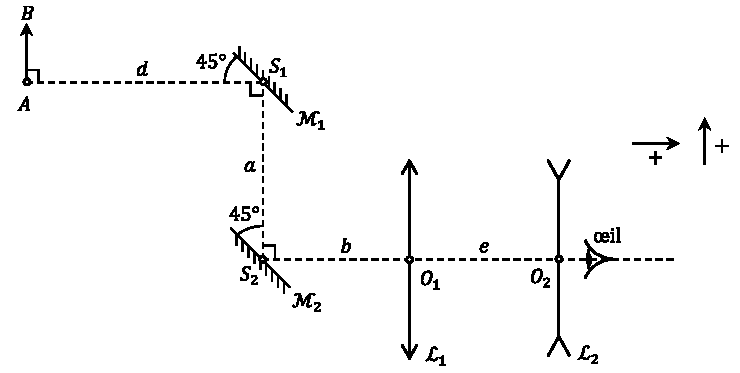
\includegraphics[width=\linewidth]{peri_plain}
			\captionof{figure}{Schéma du périscope.}
			\label{fig:peri_plain}
		\end{center}
	\end{tcb}
}%

\QR[3]{\label{q:intro}%
	Justifier simplement que le système est équivalent à une observation de
	$\mathrm{AB}$ sur un seul axe optique. Donner alors la distance
	$\mathrm{AO_1}$ et dessiner le schéma équivalent.
}{%
	Dans cet exercice, les deux miroirs ne font que renvoyer l'objet AB à une
	distance $\mathrm{AO_1} = a+b+d$ \pt{1} de la lentille 1. En effet, un miroir
	ne \textbf{modifie pas les distances} \pt{1} objet-image mais juste l'angle.
	En faisant continuer le rayon de $\mathrm{S_1}$ à $\mathrm{S_2}$ par le miroir
	$\Mc_1$ (dans le «~monde miroir~»), on garde le même fonctionnement
	géométrique, et de même pour $\Mc_2$. On se retrouve alors avec le simple
	problème de lunette terrestre suivant~:
	\begin{figure}[htbp!]
		\centering
		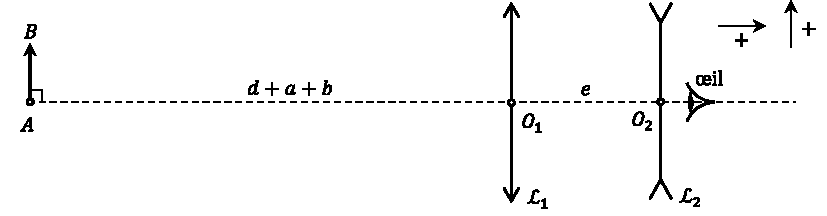
\includegraphics[scale=1]{peri_lunet}
		\caption{Schéma simplifié \protect \pt{1}}
		\label{fig:peri_lunet}
	\end{figure}
}%

\enonce{%
	\begin{tcn}(impo)<lft>{}
		Pour les questions suivantes, indiquer la ou les bonnes réponses clairement
		et en toutes lettres («~Réponse X~»), en justifiant entièrement votre choix.
	\end{tcn}
}%

\QR[9]{%
	L'objet $\mathrm{AB}$ est placé à grande distance du périscope, suffisamment
	loin pour que $d$ puisse être considéré infini. On note $e_0$ la valeur de $e$
	permettant à l'œil d'observer $\mathrm{AB}$ à travers $\Sc_p$ sans accommoder.
	Exprimer $e_0$~:
	\begin{tasks}[label=\Alph*)](4)
		\task $e_0 = f_1'-f_2'$
		\task $e_0 = f_1'$
		\task $e_0 = f_2'$
		\task $e_0 = f_1' + f_2'$
	\end{tasks}
}{%
	\textbf{Réponse D}.
	On représente la situation avec un schéma de principe \pt{1}~:
	\begin{center}
		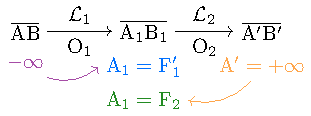
\includegraphics[scale=1]{afocal}
	\end{center}
	En effet, avec $\mathrm{AB}$ à l'infini, son image se situe dans le plan focal
	image $\pi_1'$ de $\Lc_1$, soit $\boxed{\mathrm{A_1 = F_1'}}$ \pt{1}. De plus,
	un œil emmétrope voit net sans accommoder un objet provenant de l'infini
	\pt{1}, donc l'image finale $\mathrm{A'B'}$ par $\Sc_p$ doit être à l'infini.
	Pour cela, l'image intermédiaire doit se situer dans le plan focal objet
	$\pi_2$ de $\Lc_2$, soit $\boxed{\mathrm{A_1=F_2}}$ \pt{1}~: c'est un
	\textbf{système afocal} \pt{1} avec $\mathrm{F_1' = F_2}$. Ainsi,
	\begin{DispWithArrows*}
		e_0 &\stm{=} \obarr{O_1O_2}
		\Arrow{On décompose}
		\\\Lra
		e_0 &=
		\underbracket[1pt]{\obarr{O_1F_1'}}_{=f_1' \pt{1}} +
		\underbracket[1pt]{\obarr{F_1'O_2}}_{= \obarr{F_2O_2}}
		\Arrow{$\obarr{F_2O_2} = \obarr{O_2F_2'}$ \pt{1}}
		\\\Lra
		\Aboxed{e_0 &\stm{=} f_1' + f_2'}
	\end{DispWithArrows*}
}%

\QR[9]{%
	\textbf{Question difficile mais indépendante de la suite}.
	L'objet étant encore à l'infini, on règle $\Sc_p$ de telle sorte que $e = e_0
		- \ep$, où $\ep > 0$, $\ep \ll \abs{f_2'}$ et $\ep \ll \abs{f_1'}$.
	On donne le développement asymptotique (approximation) suivant~:
	$\boxed{\DS\frac{1}{1+x} \Sim_{x \ll 1} 1-x}$. Que peut-on affirmer~?
	\begin{tasks}[label=\Alph*)](2)
		\task L'image de AB par $\Sc_p$ est réelle.
		\task L'image de AB par $\Sc_p$ est virtuelle.
		\task L'œil peut observer une image nette à travers $\Sc_p$.
		\task L'œil ne peut pas observer d'image nette à travers $\Sc_p$.
	\end{tasks}
}{%
	\textbf{Réponses B et C}.
	AB étant encore à l'infini, on a toujours $\mathrm{A_1B_1}$ située en $F_1'$.
	La relation de conjugaison de la seconde lentille donne~:
	\begin{DispWithArrows*}[groups]
		\frac{1}{f_2'} &\stm{=}
		\frac{1}{\obarr{O_2A'}} - \frac{1}{\obarr{O_2F_1'}}
		\Arrow{On développe $\obarr{O_2F_1'}$}
		\\\Lra
		\frac{1}{f_2'} &=
		\frac{1}{\obarr{O_2A'}} -
		\frac{1}{\obarr{O_2O_1} + f_1'}
		\Arrow{$\obarr{O_2O_1} = \ep - e_0$}
		\\\Lra
		\frac{1}{f_2'} &\stm{=}
		\frac{1}{\obarr{O_2A'}} -
		\frac{1}{\ep - (\cancel{f_1'} + f_2') + \cancel{f_1'}}
		\Arrow{On change le $-$ en $+$}
		\\\Lra
		\frac{1}{f_2'} &=
		\frac{1}{\obarr{O_2A'}} +
		\frac{1}{f_2' - \ep}
		\Arrow[tikz={text width=5cm}, new-group]{On fait apparaître $\ep/f_2'$ pour
			le
			développement}
		\\\Lra
		\frac{1}{f_2'} &\stm{=}
		\frac{1}{\obarr{O_2A'}} +
		\frac{1}{f_2'\left( 1 - \frac{\ep}{f_2'} \right)}
		\Arrow[tikz={text width=5cm}]{On isole $\obarr{O_2A'}$ et on développe}
		\\\Lra
		\frac{1}{\obarr{O_2A'}} &\stm{\stm(un){\approx}}
		\frac{1}{f_2'} - \frac{1}{f_2'} \left( 1+\frac{\ep}{f_2'} \right)
		\Arrow{On simplifie}
		\\\Lra
		\Aboxed{\frac{1}{\obarr{O_2A'}} &\stm{\approx} - \frac{\ep}{f_2'^2}}
	\end{DispWithArrows*}
	Ainsi, $\boxed{\obarr{O_2A'} < 0}$ \pt{1}, donc l'image se forme \textbf{avant
		$\Lc_2$}~: elle est \textbf{virtuelle}. \pt{1}
	\smallbreak
	De plus, la distance $\mathrm{O_2A}$ sera suffisamment grande pour être vue
	par l'œil \textbf{en accommodant}. \pt{1}
}%

\QR[3]{%
	L'objet est maintenant placé à distance finie. On note $\mathrm{A_1B_1}$
	l'image de $\mathrm{AB}$ par le système $\{\Mc_1,\Mc_2,\Lc_1\}$ et $p_1' =
		\obarr{O_1A_1}$. Exprimer $p_1'$~:
	\begin{tasks}[label=\Alph*)](4)
		\task $\DS p_1' = \frac{f_1' (a+b+d)}{a+b+d-f_1'}$
		\task $\DS p_1' = \frac{f_1' (a+b+d)}{a+b+d+f_1'}$
		\task $\DS p_1' = \frac{f_1' (a+b+e)}{a+b+d+f_1'}$
		\task $\DS p_1' = \frac{f_1'd}{d-f_1'}$
	\end{tasks}
}{%
	\textbf{Réponse A}.
	Grâce au schéma de la Question~\ref{q:intro}, la relation de conjugaison pour
	$\Lc_1$ donne
	\begin{DispWithArrows*}[]
		\frac{1}{f_1'} &\stm{=} \frac{1}{p_1'} - \frac{1}{-(d+a+b)}
		\Arrow{On isole $p_1'$}
		\\\Lra
		\frac{1}{p_1'} &= \frac{1}{f_1'} - \frac{1}{d+a+b}
		\Arrow{On met sur même dénominateur}
		\\\Lra
		\frac{1}{p_1'} &\stm{=} \frac{d+a+b-f_1'}{f_1'(d+a+b)}
		\Arrow{On inverse}
		\\\Lra
		\Aboxed{p_1' &\stm{=} \frac{f_1'(d+a+b)}{d+a+b-f_1'}}
	\end{DispWithArrows*}
}%

\QR[3]{%
	Quelle est alors la taille (grandeur algébrique) $\obarr{A_1B_1}$ de cette
	image intermédiaire~?
	\begin{tasks}[label=\Alph*), label-width=2ex](2)
		\task $\DS \obarr{A_1B_1} = \frac{f_1'}{f_1'+a+b+d}\obarr{AB}$
		\task $\DS \obarr{A_1B_1} = \frac{f_1'}{f_1'+f}\obarr{AB}$
		\task $\DS \obarr{A_1B_1} = \frac{f_1'}{f_1'-d}\obarr{AB}$
		\task $\DS \obarr{A_1B_1} = \frac{f_1'}{f_1'-a-b-d}\obarr{AB}$
	\end{tasks}
}{%
	\textbf{Réponse D}.
	Avec le grandissement, on a
	\begin{DispWithArrows*}
		\gamma =
		\frac{\obarr{A_1B_1}}{\obarr{AB}} &\stm{=}
		\frac{\obarr{O_1A_1}}{\obarr{O_1A}}
		\Arrow{On remplace par les distances}
		\\\Lra
		\obarr{A_1B_1} &\stm{=} \frac{p_1'}{-(a+b+d)}\obarr{AB}
		\Arrow{$p_1' = \frac{f_1'(d+a+b)}{d+a+b-f_1'}$}
		\\\Lra
		\obarr{A_1B_1} &= \frac{-f_1'}{a+b+d-f_1'}\obarr{AB}
		\Arrow{On réarrange}
		\\\Lra
		\Aboxed{\obarr{A_1B_1} &\stm{=} \frac{f_1'}{f_1'-a-b-d}\obarr{AB}}
	\end{DispWithArrows*}
}%

\QR[4]{%
	L'image $\obarr{A'B'}$ de $\mathrm{AB}$ par $\Sc_p$ se forme maintenant en
	avant de $\Lc_2$, à une distance $\obarr{A'O_2} = d_m$, avec $d_m =
		\SI{25}{cm}$, et telle que $\obarr{A'B'} = \SI{1}{mm}$.
	\smallbreak
	On note $\th > 0$ l'angle sous lequel l'image $\mathrm{AB}$ par $\Sc_p$ est
	vue par l'observataire (on rappelle que l'œil est derrière et à proximité
	immédiate de $\Lc_2$). Que peut-on affirmer~?
	\begin{tasks}[label=\Alph*)](4)
		\task $\th \approx \SI{e-3}{rad}$
		\task $\th \approx \SI{4e-3}{rad}$
		\task L'image est ponctuelle pour l'œil.
		\task L'image est étendue pour l'œil.
	\end{tasks}
}{%
	\textbf{Réponses B et D}.
	L'angle $\th$ sous lequel est vu $\mathrm{A'B'}$ est tel que, en utilisant
	l'approximation des petits angles (le système est dans les conditions de
	\textsc{Gauss} \pt{1})~:
	\begin{gather*}
		\tan(\th) \approx \th \stm{=} \frac{\obarr{A'B'}}{d_m}
		\qav
		\left\{
		\begin{array}{rcl}
			\obarr{A'B'} & = & \SI{1}{mm}
			\\
			d_m          & = & \SI{250}{mm}
		\end{array}
		\right.\\
		\AN
		\xul{
			\th \stm{\approx} \SI{4e-3}{rad}
		}
	\end{gather*}
	Ceci est plus de dix fois plus grand que le pouvoir de résolution de l'œil
	$\th\ind{min} = \SI{3e-4}{rad}$ \pt{1}. Ainsi l'image est étendue.
}%

\QR[4]{%
	Pour un objet à distance infinie, de quelle distance $\Delta{e} > 0$ faut-il
	déplacer $\Lc_2$ depuis la position précédente pour retrouver le réglage
	initial $e = e_0$~?
	\begin{tasks}[label=\Alph*)](4)
		\task $\Delta{e} = \SI{1.0}{mm}$
		\task $\Delta{e} = \SI{1.25}{cm}$
		\task $\Delta{e} = \SI{5.0}{cm}$
		\task $\Delta{e} = \SI{12.5}{cm}$
	\end{tasks}
}{%
	\textbf{Réponse D}.
	L'image intermédiaire revient en $F_1'$. Depuis la situation précédente où
	$\obarr{O_2A'} = -d_m$, on a $e = e_0 + \Delta{e}$ avec $\Delta{e}$ à trouver.
	Ainsi, avec 3 chiffres significatifs pour répondre à la question,
	\begin{DispWithArrows*}[groups]
		\frac{1}{f_2'} &\stm{=} \frac{1}{-d_m} - \frac{1}{\obarr{O_2F_1'}}
		\Arrow{$\obarr{O_2F_1'} = \obarr{O_2O_1} + \obarr{O_1F_1'}$}
		\\\Lra
		\frac{1}{f_2'} &= -\frac{1}{d_m} - \frac{1}{-(e_0+\Delta{e})+f_1'}
		\Arrow{$e_0 = f_1' + f_2'$}
		\\\Lra
		\frac{1}{f_2'} &= -\frac{1}{d_m} -
		\frac{1}{-(\cancel{f_1'}+f_2'+\Delta{e})+\cancel{f_1'}}
		\Arrow{On isole $\Delta{e}$}
		\\\Lra
		\frac{1}{f_2'+\Delta{e}} &\stm{=} \frac{1}{f_2'} + \frac{1}{d_m}
		\Arrow{Même dénominateur}
		\\\Lra
		\frac{1}{f_2'+\Delta{e}} &= \frac{d_m + f_2'}{f_2'd_m}
		\Arrow[tikz={text width=5cm}]{On inverse, isole, puis même dénominateur}
		\\\Lra
		\Delta{e} &=
		\frac{f_2'd_m}{d_m+f_2'} - f_2' \times \frac{d_m+f_2'}{d_m+f_2'}
		\\\Lra
		\Aboxed{\Delta{e} &\stm{=} \frac{-f_2'^2}{d_m+f_2'}}
		\qav
		\left\{
		\begin{array}{rcl}
			f_2' & = & \SI{-0.125}{m}
			\\
			d_m  & = & \SI{25e-2}{m}
		\end{array}
		\right.\\
		\AN
		\makebox[0pt][l]{$\xul{\phantom{\Delta{e} = \SI{1.25e-1}{m}}}$}
		\Delta{e} &\stm{=} \SI{1.25e-1}{m}
	\end{DispWithArrows*}
}%

\end{document}%
